\documentclass{article}
\usepackage{amssymb}
\usepackage{amsfonts}
\usepackage{amsmath}
\usepackage{tikz}
\author{Jonathan Kalsky}
\date{March 5 2026}
\title{\normalsize CSCE 222\\ \Large Homework 3}
\linespread{1.5}

\begin{document}
\maketitle
\tableofcontents
\vspace{1cm}
\section{Section 2.4}
\subsection{Question 12 - Suppose that A = \{2, 4, 6\}, B = \{2, 6\}, C = \{4, 6\}, and
D = \{4, 6, 8\}. Determine which of these sets are subsets
of which other of these sets.}
Definition: $A \subseteq B \iff \forall x (x \in A \to x \in B)$\\
A - None of the sets contain all elements of A, thus A is not a subset of B, C, or D\\
B - A is the only set that contains all elements of B, thus B is a subset of A\\
C - Only A and D contain all elements of C, thus C is a subset of A and D\\
D - None of the sets contain all elements of D, thus D is not a subset of A,B, or C
\subsection{Question 14 - For each of the sets in Exercise 13, determine whether
\{2\} is an element of that set.}
Definition: $A \subseteq B \iff \forall x (x \in A \to x \in B)$\\
\subsection[a]{a - \{$x \in R \; \vert $ x is an integer greater than 1\}}
Becasue all elements of \{2\} are real numbers and integers greater than 1, \{2\} is an element of that set.
\subsection[b]{b - \{$x \in R \; \vert $ x is the square of an integer\}}
There exists an element, 2, in \{2\} that is not the square of an integer as $\sqrt{2} \notin Z$. Thus \{2\} is not an element of that set.
\subsection[c]{c- \{2,\{2\}\}}
There exists an element in \{2,\{2\}\} that is equivalent to \{2\}, thus \{2\} is an element of that set by definition.
\subsection[d]{d- \{\{2\}, \{\{2\}\}\}}
There exists an element in \{\{2\}, \{\{2\}\}\} that is equivalent to \{2\}, thus \{2\} is an element of that set by definition.
\subsection[e]{e- \{\{2\}, \{2,\{2\}\}\}}
There exists an element in \{\{2\}, \{2,\{2\}\}\} that is equivalent to \{2\}, thus \{2\} is an element of that set by definition.
\subsection[f]{f- \{\{\{2\}\}\}}
By exhaustion, there does not exist an element in \{\{\{2\}\}\} that is equivalent to \{2\}, thus \{2\} is not an element of that set by definition.

\subsection{Question 22a - Use a Venn diagram to illustrate the relationships A $\subset$ B and A $\subset$ C}
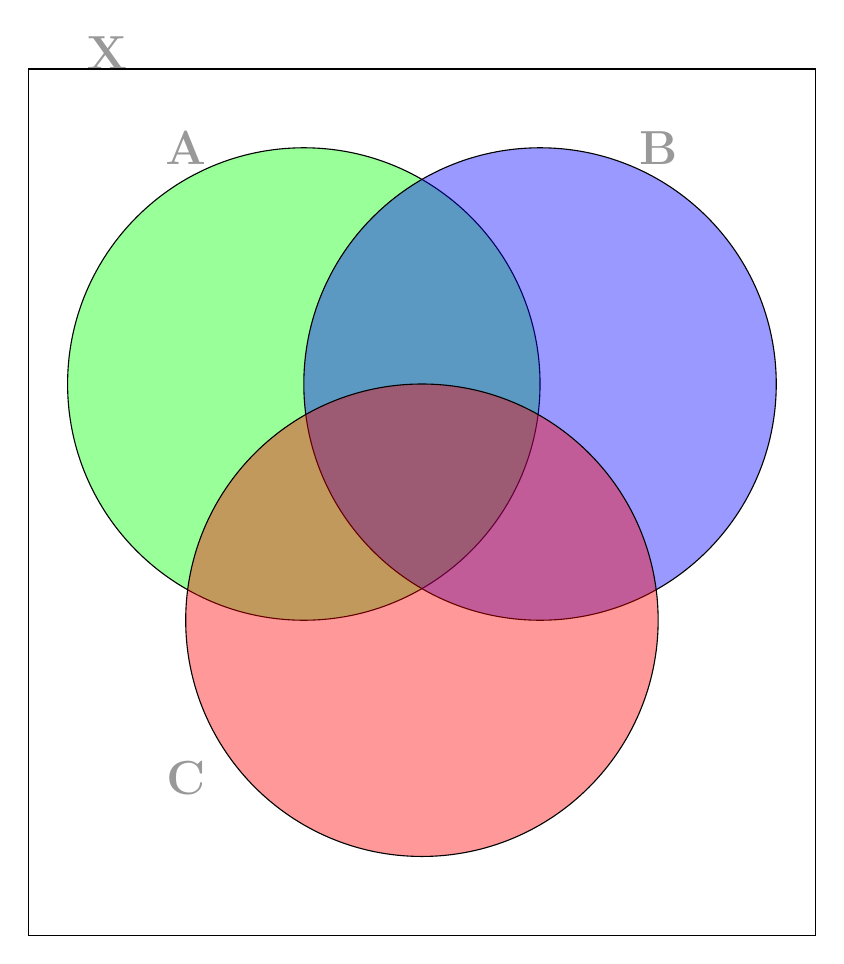
\begin{tikzpicture}
%% You can adjust the opacity here. For venn diagrams it is convenient to have a low opacity so that you can see intersections
	\begin{scope} [fill opacity = .4]
%% The draw command knows a lot of shapes. To make a rectangle you just need to specify two diagonal corners. Make sure you always have a semicolon at the end of your draw commands, otherwise latex flips out.
    \draw (-5,5) rectangle (5,-6);
%% Similarly, you can make a circle by specifying the center and then the radius. You can also add a fill color, but if you're printing in black and white you'll probably want to remove that line.
    \draw[fill=green, draw = black] (-1.5,1) circle (3);
    \draw[fill=blue, draw = black] (1.5,1) circle (3);
    \draw[fill=red, draw = black] (0,-2) circle (3);
%% We can use the node command to label points. If you put your cursor on "LARGE" or "textbf" a box will drop down with size and text style options.
    \node at (-4,5.2) {\LARGE\textbf{X}};
    \node at (-3,4) {\LARGE\textbf{A}};
    \node at (3,4) {\LARGE\textbf{B}};
    \node at (-3,-4) {\LARGE\textbf{C}};
    \end{scope}
%% And now you have a venn diagram. Yay!
%\draw[help lines](-5,5) grid (5,-6);    This line can draw the grid lines to help guide you. I use these when I'm writing the code and then delete this line when I publish the pdf.
\end{tikzpicture}
\subsection{Question 22b}
\subsection{Question 32}

\section{Section 5.1}
\subsection{Question 8}
\subsection{Question 12}
\subsection{Question 14}
\subsection{Question 18}

\end{document}